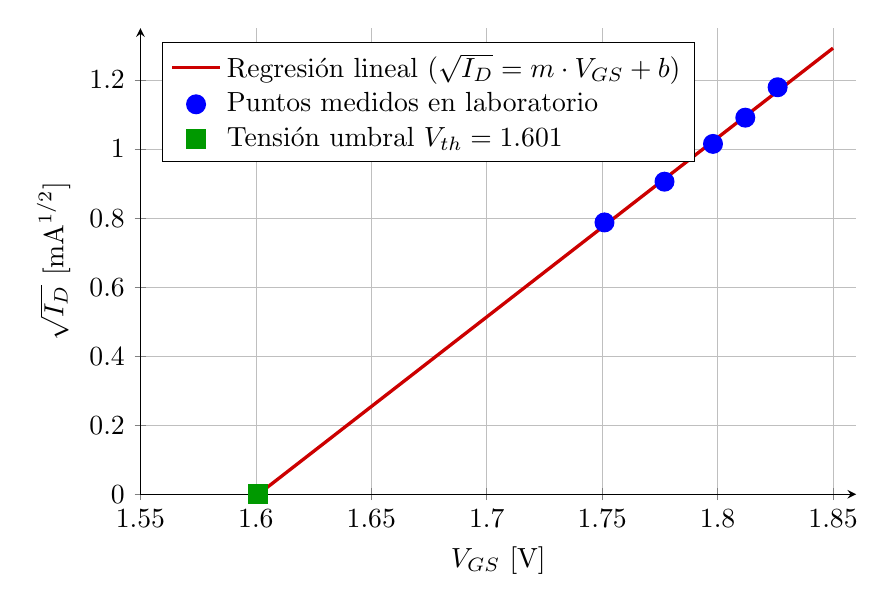
\begin{tikzpicture}
  \begin{axis}[
    width=0.88\textwidth,
    height=7.5cm,
    xlabel={$V_{GS}\ [\mathrm{V}]$},
    ylabel={$\sqrt{I_D}\ [\mathrm{mA}^{1/2}]$},
    xmin=1.55, xmax=1.86,
    ymin=0, ymax=1.35,
    grid=both,
    grid style={line width=.1pt, draw=gray!30},
    major grid style={line width=.2pt, draw=gray!50},
    axis lines=left,
    legend pos=north west,
    legend cell align={left},
    every axis plot/.append style={very thick}
  ]
    % Recta de regresion lineal: y = 5.1916 * x - 8.3121
    \addplot[domain=1.60104:1.85, color=red!80!black, samples=2] {5.1916*x - 8.3121};
    \addlegendentry{Regresión lineal ($\sqrt{I_D} = m \cdot V_{GS} + b$)}

    % Puntos medidos en laboratorio (Hoja 2)
    \addplot[only marks, mark=*, mark size=3pt, color=blue] coordinates {
      (1.751, 0.7874)
      (1.777, 0.9055)
      (1.798, 1.0149)
      (1.812, 1.0909)
      (1.826, 1.1790)
    };
    \addlegendentry{Puntos medidos en laboratorio}

    % Marcador del Vth en y = 0
    \addplot[only marks, mark=square*, mark size=3pt, color=green!60!black] coordinates {
      (1.60104, 0.0)
    };
    \addlegendentry{Tensión umbral $V_{th} = 1.601\V$}

  \end{axis}
\end{tikzpicture}
